\documentclass{ctexart}
\usepackage{geometry}
\usepackage{listings}
\usepackage{textcomp}
\usepackage{subfigure}
\usepackage{wrapfig}
\usepackage{stfloats}
\usepackage{abstract}
\renewcommand{\abstractnamefont}{\Large\bfseries}
\usepackage{float}
\usepackage{graphicx}
\usepackage{booktabs}%表格下划线
\usepackage[hidelinks]{hyperref}
\usepackage{hyperref}
\usepackage{appendix}
\usepackage{multirow}
\usepackage[lined,boxed,commentsnumbered]{algorithm2e}
\usepackage{amsmath,amssymb,amsfonts}
\usepackage[framed,numbered,autolinebreaks,useliterate]{mcode}
%记得用xelatex
% 导入首行缩进用的宏包
\usepackage{indentfirst}
\setlength{\parindent}{2em}
%标题大写,次级小写
\renewcommand\thesection{\zhnum{section}}
\renewcommand{\thesubsection}{\arabic{section}.\arabic{subsection}}
% 这里把间距设置为0.3 cm,你们可以自己调整
%\newcommand{\setParDis}{\setlength {\parskip} {0.3cm} }
\title{\textbf{应用数学选讲大作业-A题}}
\author{冯健齐 202023092020}
\date{\today}
% //////////////////////////////////////////////////

\begin{document}
\begin{center}
    \LARGE \textbf{应用数学选讲-A题}\par
    \vspace{1em}
    \normalsize \today \quad 冯健齐 \quad 202023092020
\end{center}
\begin{abstract}
\normalsize 现对于疫苗的研发,有假定疫苗生产需要经过CJ1工位,CJ2工位,CJ3工位,CJ4工位这四个工位流程才可以产出。每个工艺流程依次都可以处理100剂(1箱)疫苗。犹如下限制:\textbf{1}.每个工位不能同时生产不同类型疫苗,\textbf{2}.进入第一个工位安排的每类疫苗的生产顺序一旦确定就要一直保持不变,\textbf{3}.前一种类型的疫苗离开某个工位后,后一种类型的疫苗才能进入这个工位。现有YM1-YM10等10种不同类型的疫苗在这四个工位上的50次生产中花费时长的数据。 \par
对于问题一,我们用MATLAB中的\textbf{mean}求取均值,\textbf{std2}求取方差,\textbf{max}与\textbf{min}求取最值。最后绘制出所有的数据分布直方图以及得到了所有的数据。 \par
对于问题二,要求求出所有排列下用时最短的排列方式,我们采用\textbf{动态规划模型},并且提出了\textbf{俄罗斯方块}模型来确保生产过程中所有的工序都满足题目中的三个条件。我们对模型的严谨性进行了证明,此能够得到了最佳的结果与目标时长:\textbf{4,7,8,1,2,6,3,5,9,10}是最佳的生产顺序,在该顺序下,用时为\textbf{196.0001}分钟。 \par
对于问题三,我们视所有的工作时长数据呈\textbf{正态分布},且每一种疫苗的缩短时间点为上下两种疫苗生产的交接点时能够大大降低总时长,我们以此为自变量,采用\textbf{非线性规划模型},以所有正态分布概率乘积最大值为目标,求解出最小的1600种排列下的每一种方式的时间缩短方案:\textbf{4,9,10,7,8,1,2,6,3,5}概率为\textbf{1.9397e-08},且此概率原本总用时为\textbf{197.9792}分钟。\par
对于问题四,有了不同规模的生产任务与每天960分钟的工作时长限制,对于90\%的可靠性,我们采用正态分布\textbf{0.9分位数}进行估计。为了简化运算,我们按照当天生产的疫苗种类将其分成了\textbf{单独过程}与\textbf{混合过程},建立\textbf{动态规划模型}并写出计算伪代码,最后求解得到了两种最佳的排列方式:\textbf{7,2,8,4,10,5,1,9,6,3} 与\textbf{2,7,8,4,10,5,1,9,6,3}用时都是最短用时\textbf{202天213.12分钟}。\par
对于问题五,我们先用生产售价除以生产时长得到每一种疫苗的性价比,然后先生产性价比高的再生产性价比低的截止到100天,得到最后的计划是生产完\textbf{9,5,10,8,2}这5种疫苗之后再生产\textbf{33}天的\textbf{7}种类疫苗。到最后生产的总收入为\textbf{26820000}美元。\par
\vspace{1em}
\noindent{关键词:\textbf{动态规划 \quad 非线性规划 \quad 正态分布 \quad 俄罗斯方块模型 \quad 穷举算法}}
\end{abstract}
\thispagestyle{empty}
 \newpage
\pagenumbering{Roman}
\setcounter{page}{0}
\tableofcontents
\newpage
\setcounter{page}{1}
\pagenumbering{arabic}
\newpage
\section{问题重述}
新冠肺炎的传播,给世界带来了灾难,现对于疫苗的研发,有假定疫苗生产需要经过CJ1工位,CJ2工位,CJ3工位,CJ4工位这四个工位流程才可以产出。每个工艺流程依次都可以处理100剂(1箱)疫苗。为了防止混乱,某疫苗生产公司生产部门规定,每个工位不能同时生产不同类型疫苗,且疫苗生产不允许插队,即进入第一个工位安排的每类疫苗的生产顺序一旦确定就要一直保持不变,而且前一种类型的疫苗离开某个工位后,后一种类型的疫苗才能进入这个工位。\par
现有YM1-YM10等10种不同类型的疫苗需要生产。每种类型每箱(内装疫苗100剂)疫苗在每个工位上均进行了50次模拟生产,得到了这10中疫苗在50次生产中花费时长的数据。要求建立数学模型,回答下面问题: \par
\textbf{问题1}:对每箱疫苗在所有工位上的生产时间进行均值、方差、最值、概率分布的统计分析,得到各个值的数据或者图表显示。\par
\textbf{问题2}:现需YM1-YM10各100剂(1箱)疫苗进行检测。疫苗生产公司需要对疫苗的生产顺序进行规划,以便能在最短时间内交付,以每个工位生产每箱疫苗平均时间为生产时间。请建立数学模型,制定疫苗生产顺序,初始时刻为00:00,计算生产总时间,得到结果并以表格显示。\par
\textbf{问题3}:每个工位生产每种疫苗的所需时间具有随机性,服从一定的概率分布。如果要求疫苗交货总时间比问题2的总时间缩短5\%,以最大的概率完成这个任务为目标,确定生产顺序,并给出缩短的时间比例与最大概率之间的关系。\par
\textbf{问题4}:现在该疫苗生产公司接收了10种类型疫苗不同规模的生产任务。由于生产机器需要检修和维护,每个工位每天生产的时间不能超过16小时。为避免疫苗错误包装,要求同种类型疫苗生产全部完成之后才能生产另外类型的疫苗。在可靠性为90\%的前提下安排生产方案,建立数学模型并求解至少多少天可以完成任务\par
\textbf{问题5}:如果该疫苗生产公司计划在100天内选择部分数量的疫苗进行生产,且每个工位每天生产的时间不能超过16小时,每种类型的疫苗可以只完成一部分,以最大销售额为目标,建立数学模型安排生产计划。\par

\section{问题分析}
\subsection{问题一的分析}
第一题中,要求对数据进行分析,即对表格中的数据求均值,方差,最值与概率分布,我们用MATLAB中的\textbf{mean}求取均值,\textbf{std2}求取方差,\textbf{max}与\textbf{min}求取最值,\textbf{histogram}绘制分布直方图。
\subsection{问题二的分析}
对于问题二,每个工位不能同时生产不同类型疫苗,且疫苗生产不允许插队,前一种类型的疫苗离开工位后,后一种类型的疫苗才能进入这个工位。由于题目中的的条件约束,我们采用\textbf{动态规划\cite{ref2}},建立\textbf{俄罗斯方块模型}来计算所有的组合方式以选择其中总时长最短的方案。
\subsection{问题三的分析}
对于问题三,对于缩短5\%的时长,我们采用\textbf{非线性规划模型},视生产时间分布呈正态分布,以最大概率为目标进行规划,计算出最佳的缩短时间,然后再带入不同的缩短时间,计算出最大概率,得到最后的缩短比例与最大概率的关系。
\subsection{问题四的分析}
对于问题四,需要大规模的生产且有每天的工作时长限制,我们建立以用时最短为目标的规划模型,由于一次只能生产一种类型的疫苗,为了简化算法,我们将过程分为单独过程与混合过程,更快速的算出所有排列下的用时,并进行记录与求最小值。
\subsection{问题五的分析}
对于问题五,可以指完成一部分,且给出了每一种的售价,我们可以算出每一种疫苗的生产性价比,即生产单位时间所产生的价值,然后先生产\textbf{性价比}高的,再生产性价比低的,直到生产时间达到100天,最后我们可以得到最终的生产模型\cite{ref1}以得出产生收益最多的生产规划。

\section{模型假设}
\textbf{1}.基于日常的生产流水线结构,假设生产过程中完成后仍待在机器中,无法另行保存,即该疫苗进入下一工位才可以让下一种疫苗进入该工位。\par
\textbf{2}.假设每一台机器对每一种疫苗的生产时间呈正态分布,即产生的时间分布概率呈正态分布。\par
\textbf{3}.假设机器从开始工作到最后停下(一天结束)都在工作,中间不会停止歇息。\par

\section{符号说明}

\begin{table}[H]
	\centering 
	\begin{tabular}{ccc}
		\toprule
		符号 & 含义说明 & 单位 \\
		\midrule
		$a_{(i)}$ & 该种疫苗在某一序列中位于第$i$位进行生产 & \\
		$a_{(i)},j$ & 第$i$位的疫苗的第$j$阶段生产 & \\
		$t_{a_{(i)},j}$ & $a_{(i)},j$的生产时长 & 分钟 \\
		$T_{a_{(i)},j}$ & $a_{(i)},j$的生产终止时间 & 分钟 \\
		$P_i$ & 第i类疫苗每天最多生产箱数 & 箱 \\
		$rest_i$ & 第i类疫苗剩余的箱数 & 箱 \\
		$D_i$ & 第i类疫苗的生产天数 & 天 \\
		$D_{total}$ & 生产完成所需的总天数 & 天 \\
		$r_{a(i)}$ & 第$a(i)$种疫苗的生产性价比 & 美元/分钟 \\
		$w_{a(i)}$ & 第$a(i)$种疫苗的销售价格 & 美元/剂 \\
		\bottomrule
	\end{tabular}
\end{table}



\section{模型的建立与求解}
\subsection{问题一模型的建立与求解}
\subsubsection{问题一模型的建立}
我们用MATLAB中的\textbf{mean}求取均值,\textbf{std2}求取方差,\textbf{max}与\textbf{min}求取最值。
\subsubsection{问题一模型的求解与结果分析}
导入所有的数据之后,经过MATLAB的计算,我们得到表\ref{表格1}的数据,可见在所有测试的生产中,出现的时长最短的为YM4的CJ3阶段,用时5.3536,时长最长的是YM1的CJ4阶段,用时23.789分钟;每个时长的均值中,用时最短的是YM4的CJ3阶段5.93587分钟,用时最长的是YM6的CJ2阶段20.0944分钟;每个时长的方差中,最小的是YM4的CJ3阶段0.19493,最大的是YM1的CJ4阶段1.37468.

\begin{table}[!h]
    \centering
    \resizebox{\textwidth}{!}{
    \begin{tabular}{|c|c|c|c|c|c|c|c|c|}
    \hline\hline
        疫苗类型  & \multicolumn{4}{c|}{YM1}  & \multicolumn{4}{c|}{YM2} \\ \hline
        生产工位 & CJ1 & CJ2 & CJ3 & CJ4 & CJ1 & CJ2 & CJ3 & CJ4 \\ \hline
        最大值 & 16.5784 & 17.5855 & 22.908 & 23.789 & 11.6821 & 22.2294 & 20.1778 & 21.4245 \\ \hline
        最小值 & 10.0557 & 13.067 & 17.8616 & 16.5052 & 6.9708 & 17.5137 & 15.5031 & 17.1641 \\ \hline
        均值 & 13.284036 & 14.962134 & 19.846022 & 20.012922 & 9.87088 & 19.907534 & 17.928158 & 18.942358 \\ \hline 
        方差 & 1.262528917 & 1.040711667 & 1.089726857 & 1.374675342 & 0.912844245 & 1.119335195 & 0.949834206 & 0.943654882 \\ \hline\hline
        疫苗类型  & \multicolumn{4}{c|}{YM3} & \multicolumn{4}{c|}{YM4} \\ \hline
        生产工位 & CJ1 & CJ2 & CJ3 & CJ4 & CJ1 & CJ2 & CJ3 & CJ4 \\ \hline
        最大值 & 21.814 & 17.8089 & 17.7873 & 17.0034 & 10.0389 & 12.5088 & 6.3889 & 20.7891 \\ \hline
        最小值 & 17.814 & 13.978 & 12.671 & 12.8065 & 5.872 & 7.6405 & 5.3536 & 16.0432 \\ \hline
        均值 & 20.058414 & 15.97263 & 14.970352 & 15.116388 & 7.988652 & 9.936646 & 5.935868 & 18.128398 \\ \hline
        方差 & 0.919125009 & 0.832702936 & 1.019822179 & 0.901205934 & 0.965490089 & 0.976417415 & 0.19492674 & 1.061939536 \\ \hline\hline
        疫苗类型  & \multicolumn{4}{c|}{YM5} & \multicolumn{4}{c|}{YM6} \\ \hline
        生产工位 & CJ1 & CJ2 & CJ3 & CJ4 & CJ1 & CJ2 & CJ3 & CJ4 \\ \hline
        最大值 & 10.3845 & 16.6052 & 15.0108 & 14.5267 & 21.7526 & 21.9278 & 15.8136 & 16.9491 \\ \hline
        最小值 & 5.927 & 11.7967 & 10.7985 & 9.2316 & 16.4356 & 17.5005 & 12.0908 & 11.7249 \\ \hline
        均值 & 8.770062 & 13.722012 & 13.005208 & 11.24949 & 19.07412 & 20.094358 & 14.148532 & 13.883878 \\ \hline
        方差 & 0.863185422 & 1.067506779 & 0.911757145 & 1.109426758 & 1.155415745 & 0.986646508 & 0.935659811 & 1.073187377 \\ \hline\hline
        疫苗类型  & \multicolumn{4}{c|}{YM7} & \multicolumn{4}{c|}{YM8} \\ \hline
        生产工位 & CJ1 & CJ2 & CJ3 & CJ4 & CJ1 & CJ2 & CJ3 & CJ4 \\ \hline
        最大值 & 13.2878 & 18.7304 & 14.4366 & 20.7553 & 18.0783 & 10.1871 & 21.5699 & 18.7351 \\ \hline
        最小值 & 8.8435 & 14.6801 & 9.6528 & 16.7402 & 13.5753 & 7.9676 & 16.3152 & 14.7471 \\ \hline
        均值 & 11.160148 & 16.496146 & 12.013664 & 19.087604 & 16.0201 & 8.82748 & 18.114384 & 16.831394 \\ \hline
        方差 & 1.013068014 & 0.964085394 & 0.886688065 & 0.810161883 & 1.063825743 & 0.511280282 & 1.034413526 & 0.95538933 \\ \hline\hline
        疫苗类型  & \multicolumn{4}{c|}{YM9} & \multicolumn{4}{c|}{YM10} \\ \hline
        生产工位 & CJ1 & CJ2 & CJ3 & CJ4 & CJ1 & CJ2 & CJ3 & CJ4 \\ \hline
        最大值 & 17.4124 & 14.7485 & 7.9947 & 9.8984 & 13.6186 & 8.5793 & 9.8172 & 17.4872 \\ \hline
        最小值 & 12.8237 & 10.0932 & 6.2319 & 8.1086 & 11.4639 & 5.9503 & 7.9742 & 14.9504 \\ \hline
        均值 & 15.014602 & 12.03512 & 7.041914 & 8.949654 & 12.952448 & 7.010982 & 9.04917 & 16.052406 \\ \hline
        方差 & 0.986816797 & 1.076138787 & 0.365599114 & 0.418563054 & 0.455512309 & 0.531209821 & 0.455372472 & 0.513219576 \\ \hline\hline
    \end{tabular}
    }
    \\
    \caption{数据的最值,均值与方差}
    \label{表格1}
\end{table}

接着,我们用\textbf{histogram}绘制分布直方图,得到下面的图像,可以看到每个疫苗每个生产环节的数据的分布图象。

\begin{figure}
\centerline{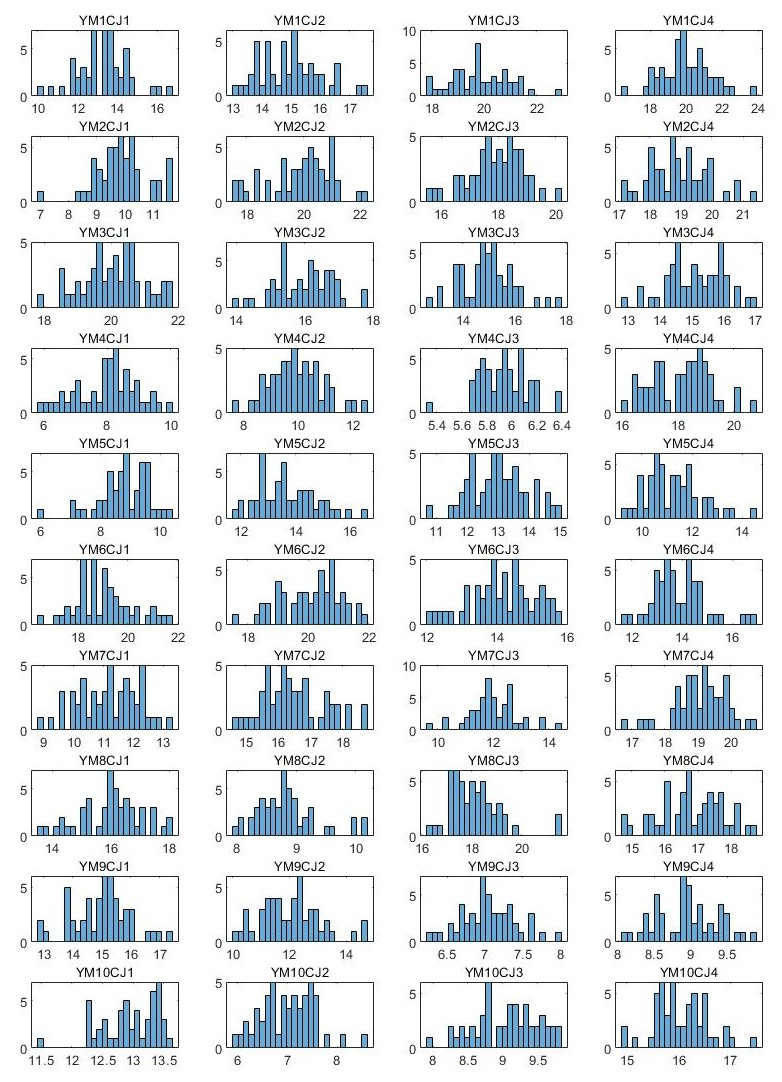
\includegraphics[width=1\linewidth]{A1图片/数据分布直方图.jpg}}
\caption{数据直方图}
\label{数据直方图}
\end{figure}

\newpage
\subsection{问题二模型的建立与求解}
\subsubsection{问题二模型的建立}
对于该类问题,我们采用\textbf{动态规划}模型\cite{ref2},即历遍所有的情况以求取时间最短的排列情况。先进行建模的模型准备,记所有的排列组合为
\begin{align}
S = \{ a_{(1)} , a_{(2)} ... , a_{(10)} \}\nonumber 
\end{align}

其中$a_{(i)}$表示第$a_{(i)}$种疫苗在该序列中位于第$i$位进行生产,且其中的元满足以下公式
\begin{equation}
    \begin{cases}
        \quad \Omega_{(1)} = \{ 1 , 2 , 3 ... , 10 \} ,\quad a_{(1)} \in \Omega_{(1)} \\
        \quad \Omega_{(2)} = \Omega_{(1)} \setminus a_{(1)} , \quad a_{(2)} \in \Omega_{(2)}\\ 
        \quad \Omega_{(3)} = \Omega_{(2)} \setminus a_{(2)} , \quad a_{(3)} \in \Omega_{(3)}\\
        \quad \vdots \\
        \quad \Omega_{(i)} = \Omega_{(i-1)} \setminus a_{(i-1)} , \quad a_{(i)} \in \Omega_{(i)},\quad i \in \{ 2 , 3 , 4 ... , 10 \} \\
        \quad \vdots\\
        \quad \Omega_{(10)} = \Omega_{(9)} \setminus a_{(9)} , \quad a_{(10)} \in \Omega_{(10)}\nonumber 
        \label{solve}
     \end{cases}
\end{equation}

可见$card(S)=A_{10}^{10}$,即所有的排列组合有3628800种。我们记位于第$i$位的疫苗的第$j$阶段生产为$a_{(i)},j$其中$j \in \{1,2,3,4\}$,下面,我们进行模型的构造:记$a_{(i)},j$的生产时长为$t_{a_{(i)},j}$(单位:分钟),记$a_{(i)},j$的生产终止时间为$T_{a_{(i)},j}$(单位:分钟),我们要求的是$T_{a_{(10)},4}$的最小值,其中的约束条件有:

\textbf{条件一:}只有按照CJ1-CJ2-CJ3-CJ4的顺序在4个工位都进行了加工以后,才算完成生产,说明$T_{a_{(i)},j} \leq T_{a_{(i)},j+1}-t_{a_{(i)},j+1}$对于$i \in \{ 1,2,3...,10\},j\in \{ 1,2,3\}$均成立。即每个疫苗的生产流程只能像如图(a)或(b)所示的阶梯状的形状,为了达到时长最短,$a_{(1)},j$肯定是按照(a)的严格阶梯排列。\par
\begin{figure}[h]  
	\centering
	\subfigure[条件一(1)]{
		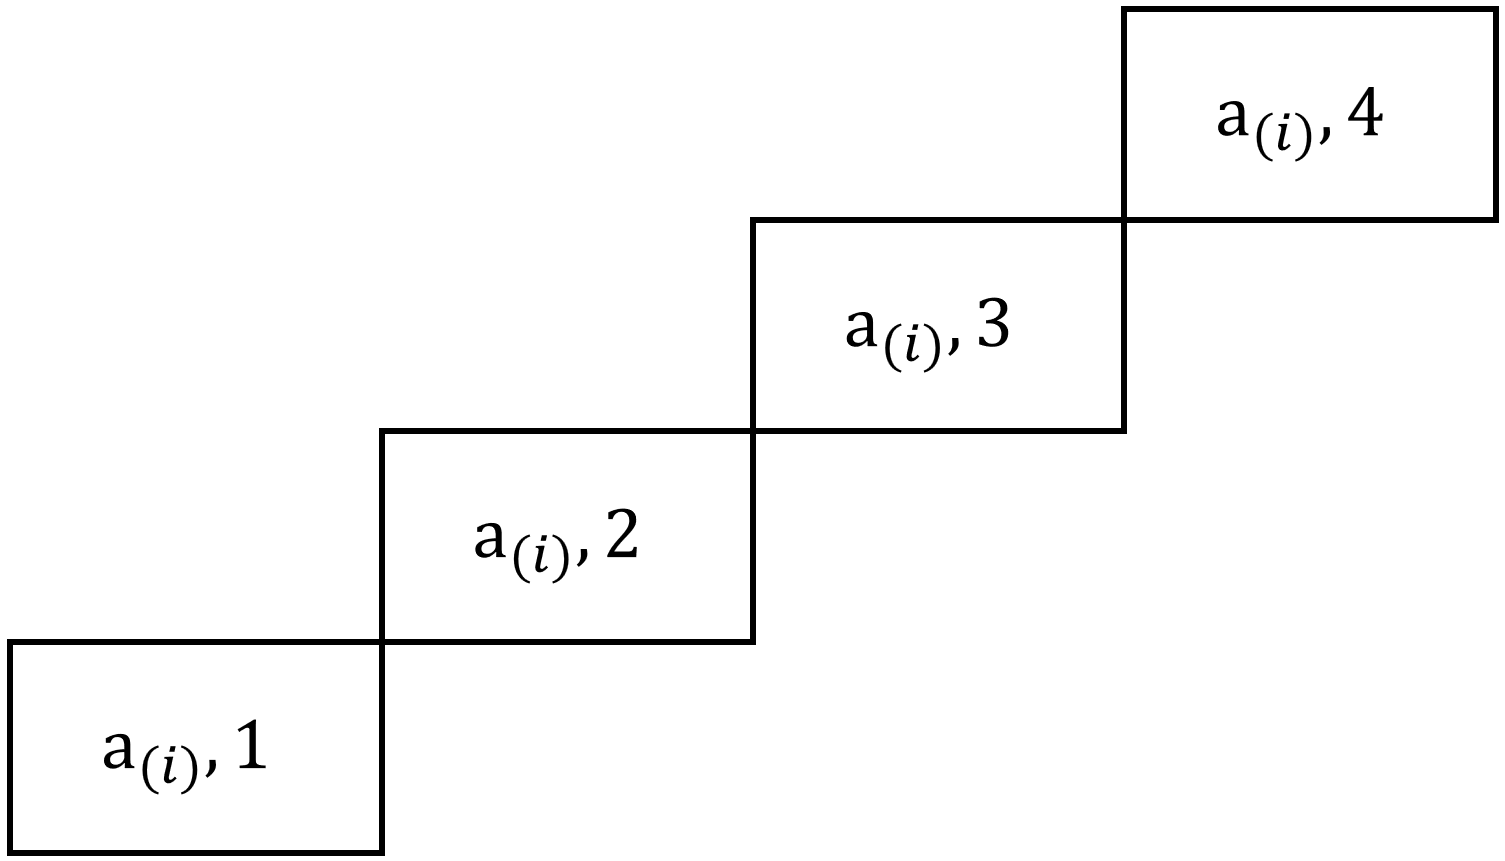
\includegraphics[width=5cm]{A2图片/process1.png}
	}
	\quad
	\subfigure[条件一(2)]{
		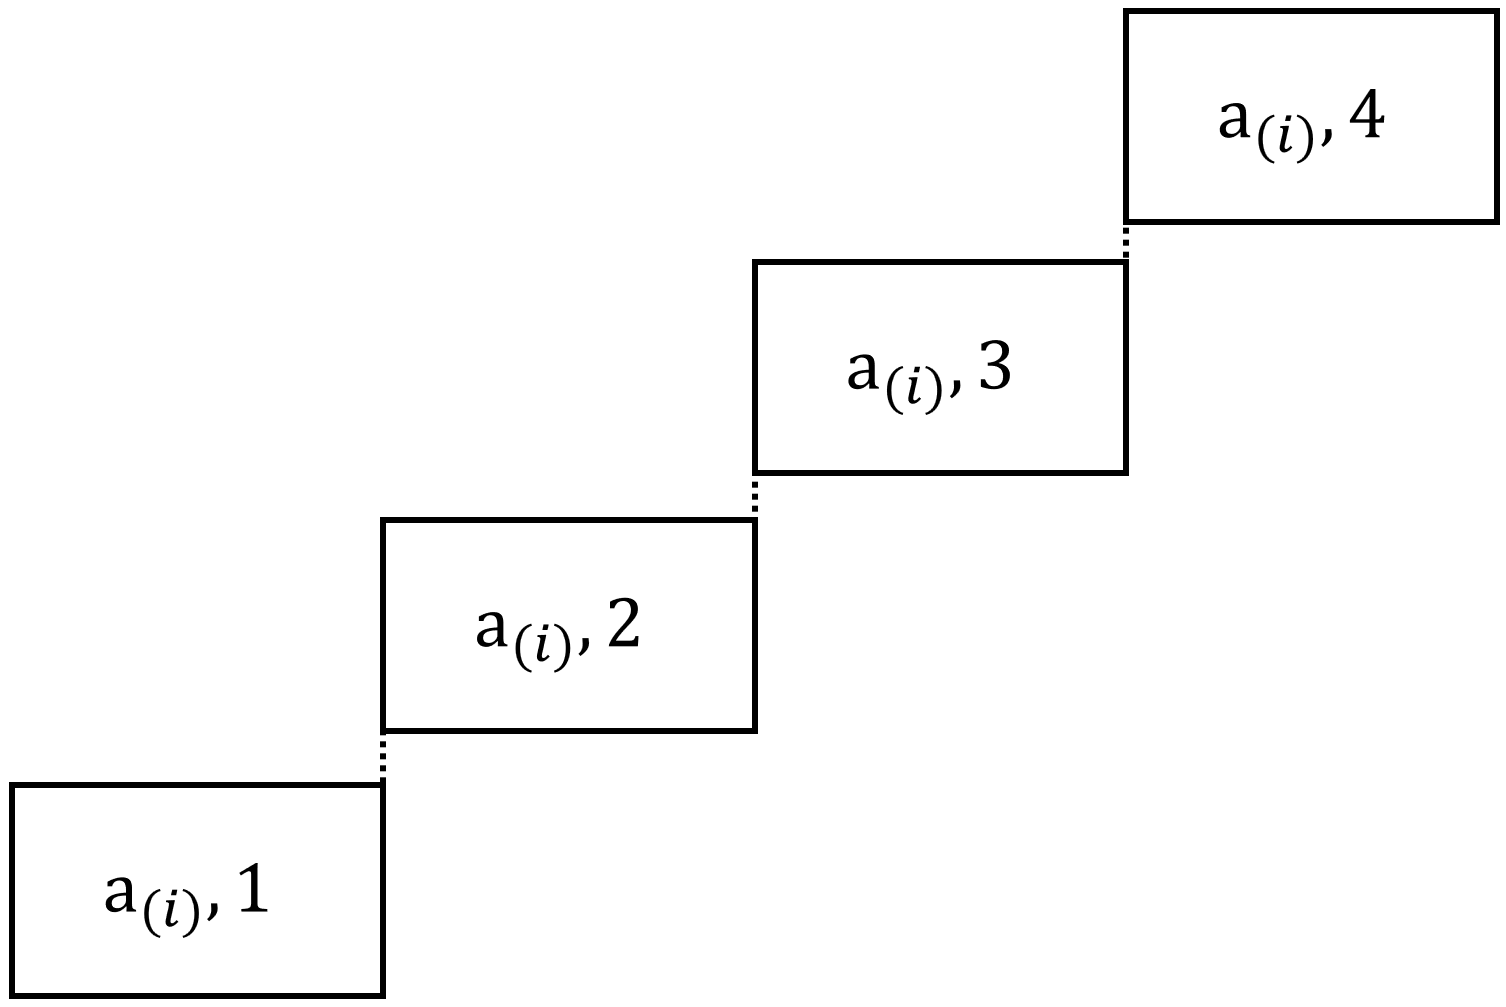
\includegraphics[width=5cm]{A2图片/process2.png}
	}
	\label{条件}
\end{figure}
\textbf{条件二:}前一种类型的疫苗离开某个工位后,后一种类型的疫苗才能进入这个工位,说明当$T_{a_{(i)},j} < T_{a_{(i)},j+1}-t_{a_{(i)},j+1}$时,为了追求最短时间,第$j$个流程处理完$a_{(i)}$疫苗后,会尽快的处理$a_{(i+1)}$疫苗,即出现如图(c)所示的情况,此时,有$T_{a_{(i+1)},j}-t_{a_{(i+1)},j} =  T_{a_{(i)},j}$,但是此时$a_{(i)},j+1$类疫苗仍在占用$j+1$工位进行制作,说明$a_{(i)}$仍然在$j$工位,而$a_{(i+1)}$已经在$j$开始生产,这与题目中的假设矛盾。所以说,只能有$T_{a_{(i)},j} = T_{a_{(i)},j+1}-t_{a_{(i)},j+1}$成立,就像图(d)中展示的一样,即每个疫苗的生产只能像图(a)所示的呈严格的阶梯状
\begin{figure}[h]  
	\centering
	\subfigure[条件二(1)]{
		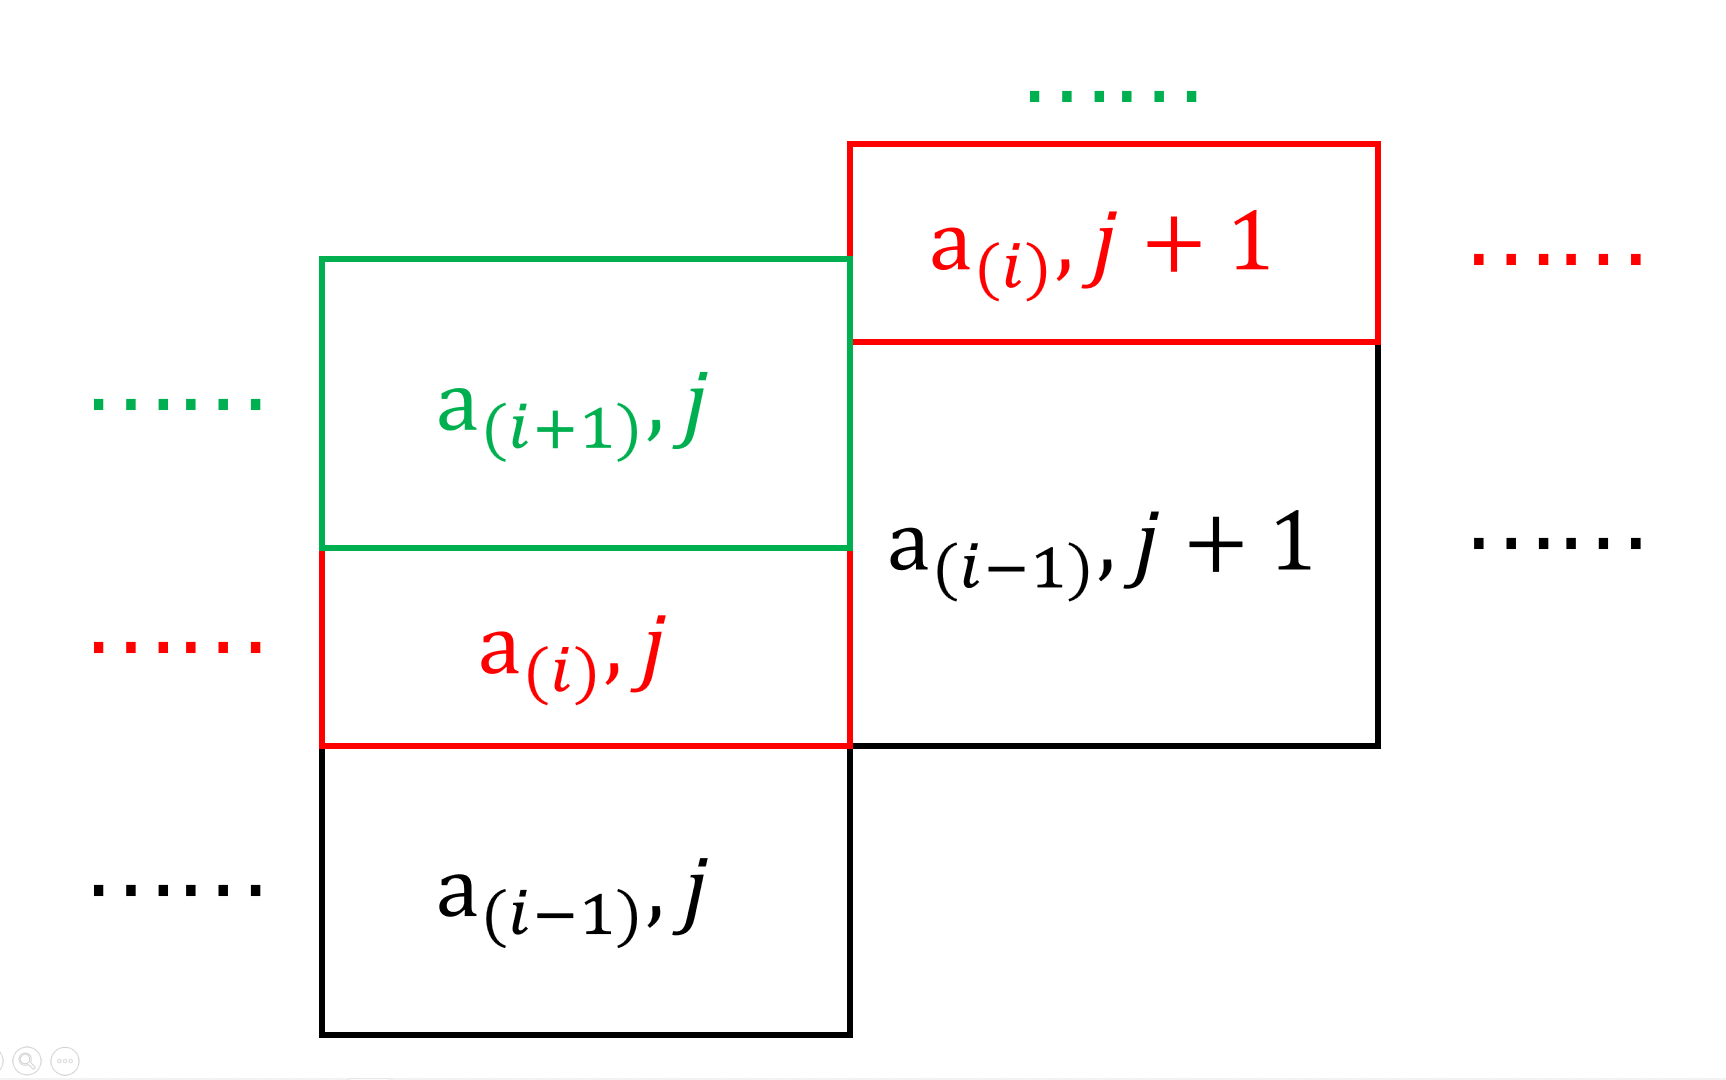
\includegraphics[width=6cm]{A2图片/process3.png}
	}
	\quad
	\subfigure[条件二(2)]{
		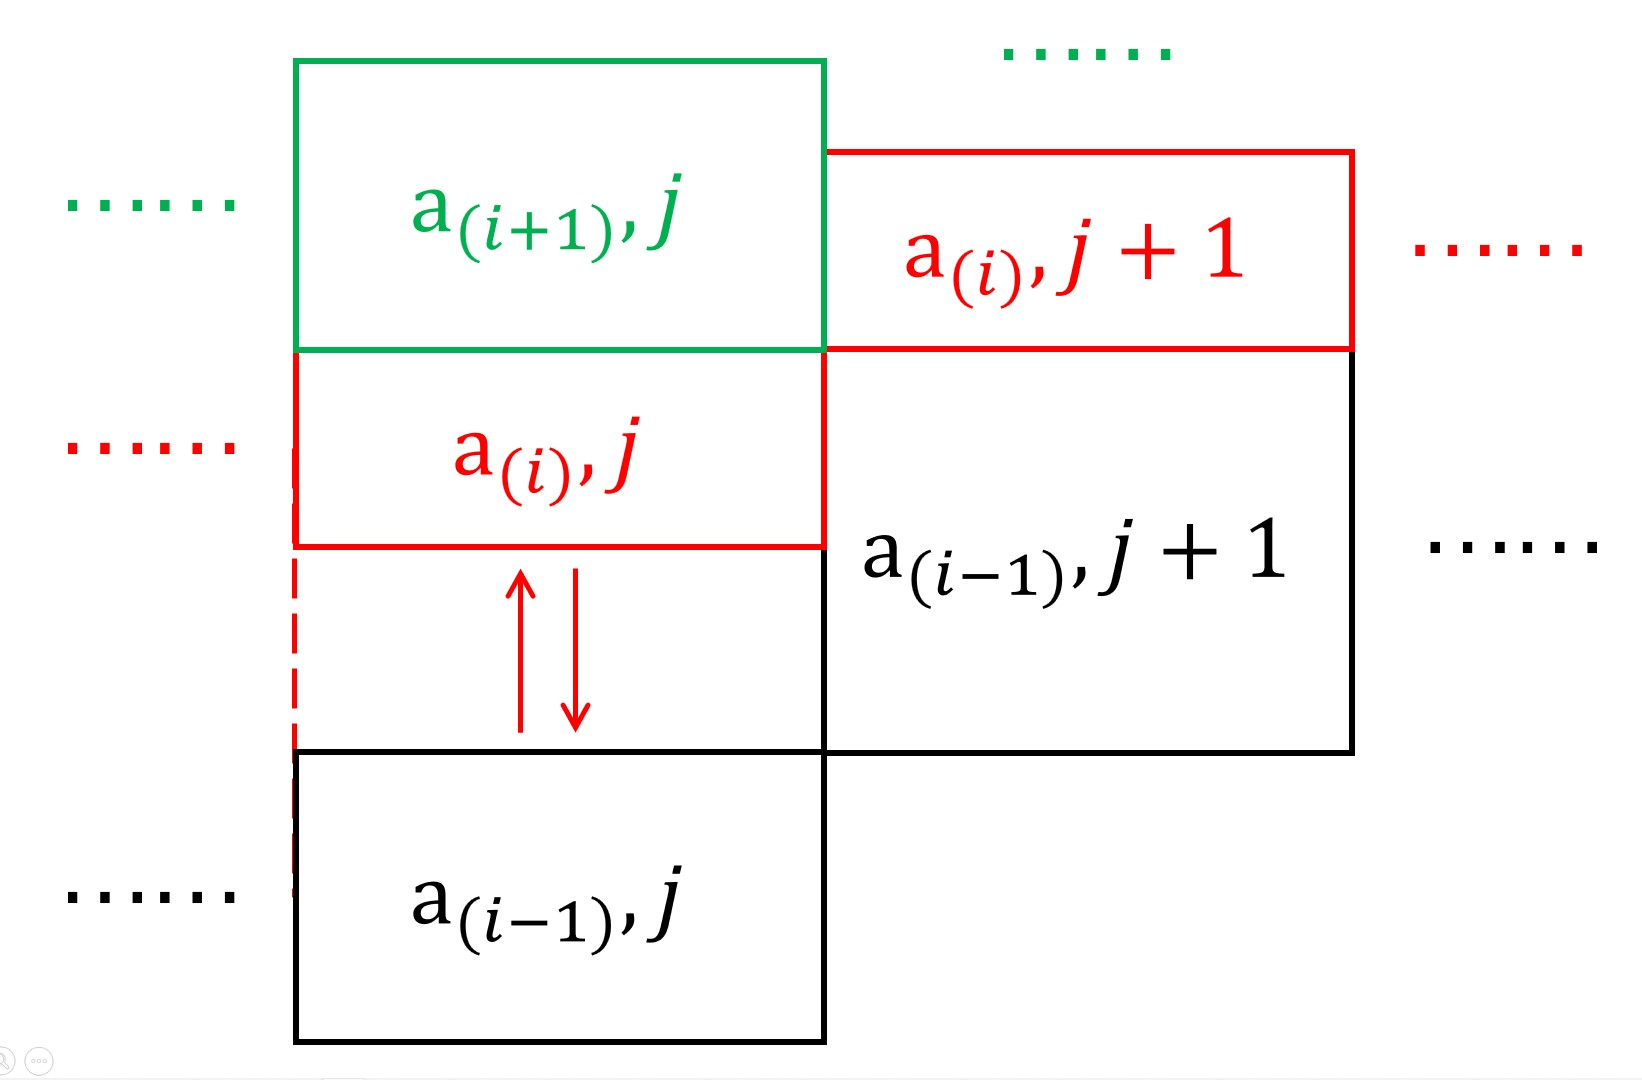
\includegraphics[width=6cm]{A2图片/process4.JPG}
	}
\end{figure}

所有的疫苗生产过程的叠加就像游戏俄罗斯方块所展示的一样,就是看怎样叠能使得总高度(总时长)最短,以达到理想状态,下面我们给出总结的动态规划模型:
\begin{align*}
&\min \quad T_{a_{(10)},4} \\
& \begin{array}{r@{\quad}l@{}l@{\quad}l}
s.t.& T_{a_{(i)},j} + t_{a_{(i)},j+1} = T_{a_{(i)},j+1}, \quad &i=1,2,3\ldots,10, \quad j=1,2,3\\
    & T_{a_{(1)},j} = \sum_{k = 1}^{j} t_{a_{(1)},k}, &j=1,2,3,4\\
& \mathop{min}\limits_{j} \{T_{a_{(i+1)},j}-t_{a_{(i+1)},j}-T_{a_{(i)},j} \} = 0, \quad &i=1,2,3\ldots,9\\
& \{ a_{(1)} , a_{(2)} ... , a_{(10)} \} \in S
\end{array}
\end{align*}

\subsubsection{问题二模型的求解}

\begin{wrapfigure}[9]{r}{0.6\textwidth}%数字来规定行数
\vspace{-5em}
  \begin{center}
    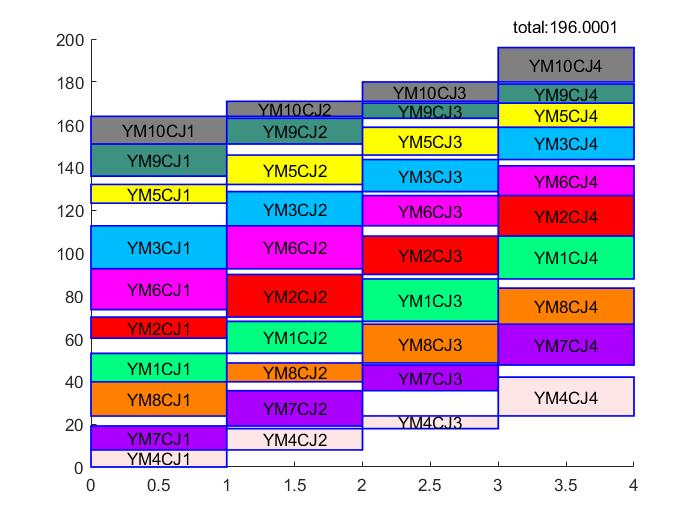
\includegraphics[width=0.6\textwidth]{A2图片/A1最短.jpg}
  \end{center}
  \label{min}
  \caption{最短用时排列模型展示}
\end{wrapfigure}

经过MATLAB动态规划的计算,我们最终得到了其中用时最短的情况,如图\ref{min}所示.可见,按照4,7,8,1,2,6,3,5,9,10的疫苗类型顺序进行生产的总用时最短,为196.0001分钟。

接着,我们计算出每种类型疫苗的开始时间与结束时间,如表\ref{问题二}所示
\begin{table}
    \centering
    \begin{tabular}{|c|c|c|}
    \hline
        \textbf{加工顺序} & \textbf{进入CJ1时刻} & \textbf{离开CJ4时刻} \\ \hline
        4 & 0 & 41.989564 \\ \hline
        7 & 7.988652 & 66.746214 \\ \hline
        8 & 23.78425 & 83.577608 \\ \hline
        1 & 39.80435 & 107.909464 \\ \hline
        2 & 60.202892 & 126.851822 \\ \hline
        6 & 73.534812 & 140.7357 \\ \hline
        3 & 92.644876 & 158.76266 \\ \hline
        5 & 123.265378 & 170.01215 \\ \hline
        9 & 135.920514 & 178.961804 \\ \hline
        10 & 150.935116 & 196.000122 \\ \hline
    \end{tabular}
    \caption{问题二结果}
    \label{问题二}
\end{table}

\newpage

后面,我们随机抽取了其中的10种情况来进行绘制,得到以下的几个样本模型:

\begin{figure}[h]
\centerline{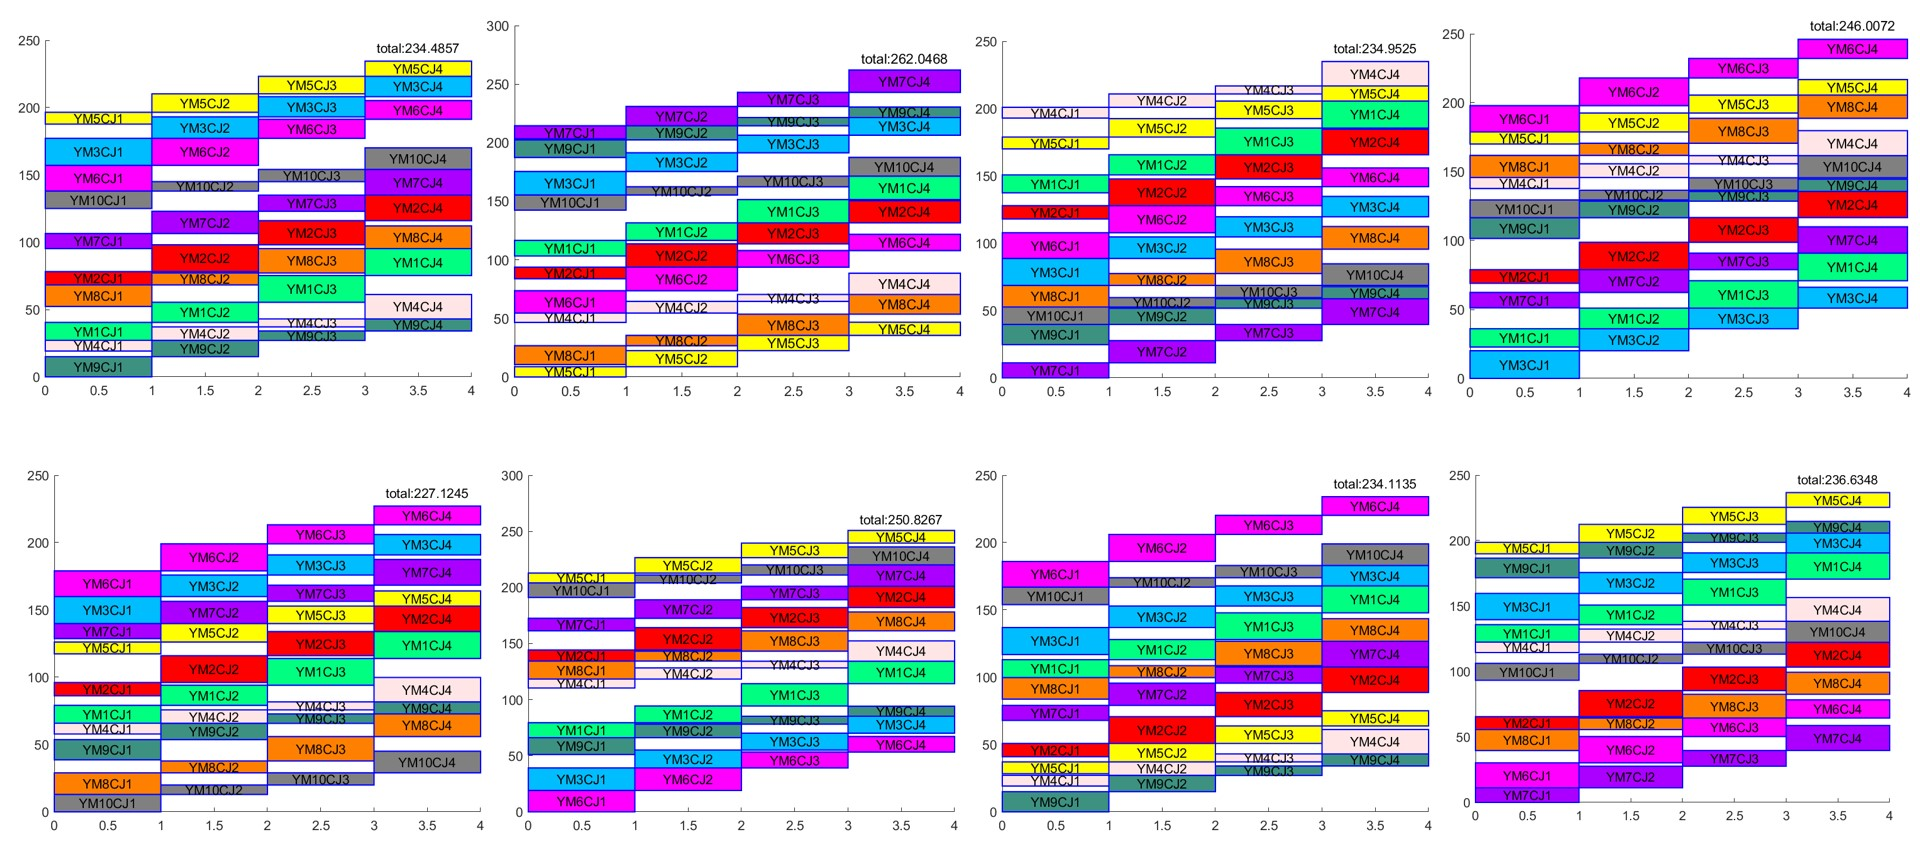
\includegraphics[width=0.9\linewidth]{A2图片/汇总8.JPG}}
\caption{样本模型图}
\label{样本}
\end{figure}
可见,该方法可以计算出所有的排列组合方式下的耗时总时长,最中得出用时最短的一个排列方式与最短的总用时。

\subsection{问题三模型的建立与求解}
\subsubsection{问题三模型的建立}
在该问题中,由于采用平均值的误差,机器有可能性会减少生产时间。而从问题一的分布直方图来看,我们假设每种疫苗每个工位的生产时间呈正态分布,且分布的均值与方差如问题一所示。这时,我们可以采用非线性规划,来计算所求的最短时间与排列方式。由问题二模型的建立过程\cite{ref2},我们知道,生产一种疫苗后生产下一种时,必然有一个机器连续工作,故只对该位置进行考虑,如图所示。\par
\begin{figure}[h]
\centerline{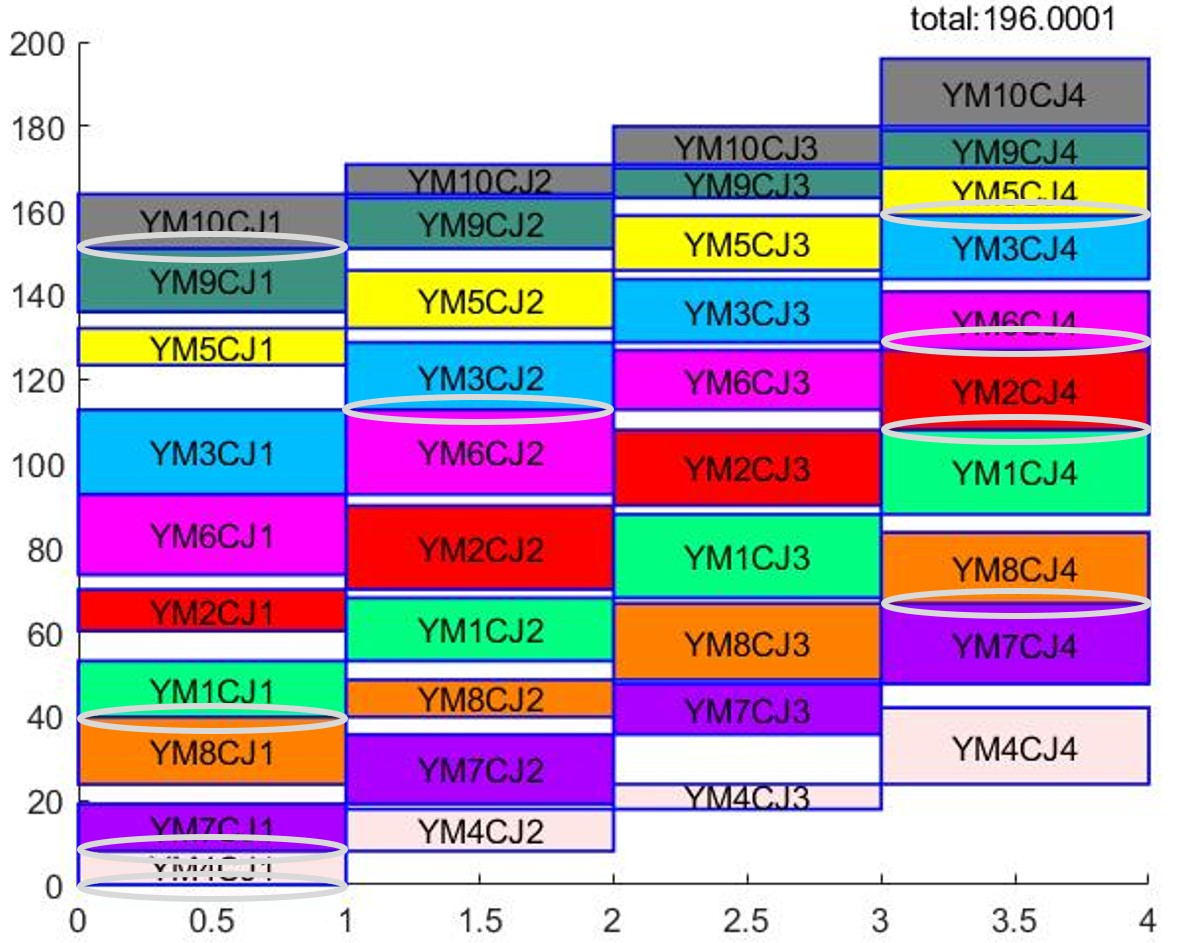
\includegraphics[width=0.55\linewidth]{A3图片/pre.JPG}}
\caption{缩短点的位置确定}
\label{pre}
\end{figure}
由于可以缩短的时间与其他三个流程生产时间有关,我们记这十种疫苗每种需要缩短的时长记为$x_i$,记缩短的最大值为$a_i$。首先,我们构造单次生产中的最大概率规划模型.
\begin{align*}
&\min \quad \sum_{i=1}^{n}\frac{1}{\sqrt{2\pi}\sigma_{i}}e^{-\frac{(x_i-\mu_i)^2}{2\sigma_{i}^2}}\\
& \begin{array}{r@{\quad}l@{}l@{\quad}l}
s.t. & \sum_{i=1}^{10}x_i = 5\%T_{min}\\
& x_i \in [0,a_i]\\
& a_i = min\{\{T_{a_{(i+1)},j}-T_{a_{(i)},j}-t_{a_{(i+1)},j}\}\setminus0\}\\ &i=1,2,3\ldots,9, \quad j=1,2,3,4\\
& \sum_{i=1}^{10}a_i \geq 5\%T_{min}
\end{array}
\end{align*}\par
\subsubsection{问题三模型的求解}
我们将这个函数带入所有的排列中,找到概率最大的,由于3628800个数据量较大,而且规划的约束有$\sum_{i=1}^{10}x_i = 5\%T_{min}$,问题二中计算出的最短用时为196.0001分钟,我们计算增加时长为5\%的数据,有1600个,这些数据降低到最短用时的5\%概率相对其余数据更大。我们将这1600个数据带入最大概率规划模型得到所有概率,如图\ref{prob}所示\par
\begin{figure}[h]
\centerline{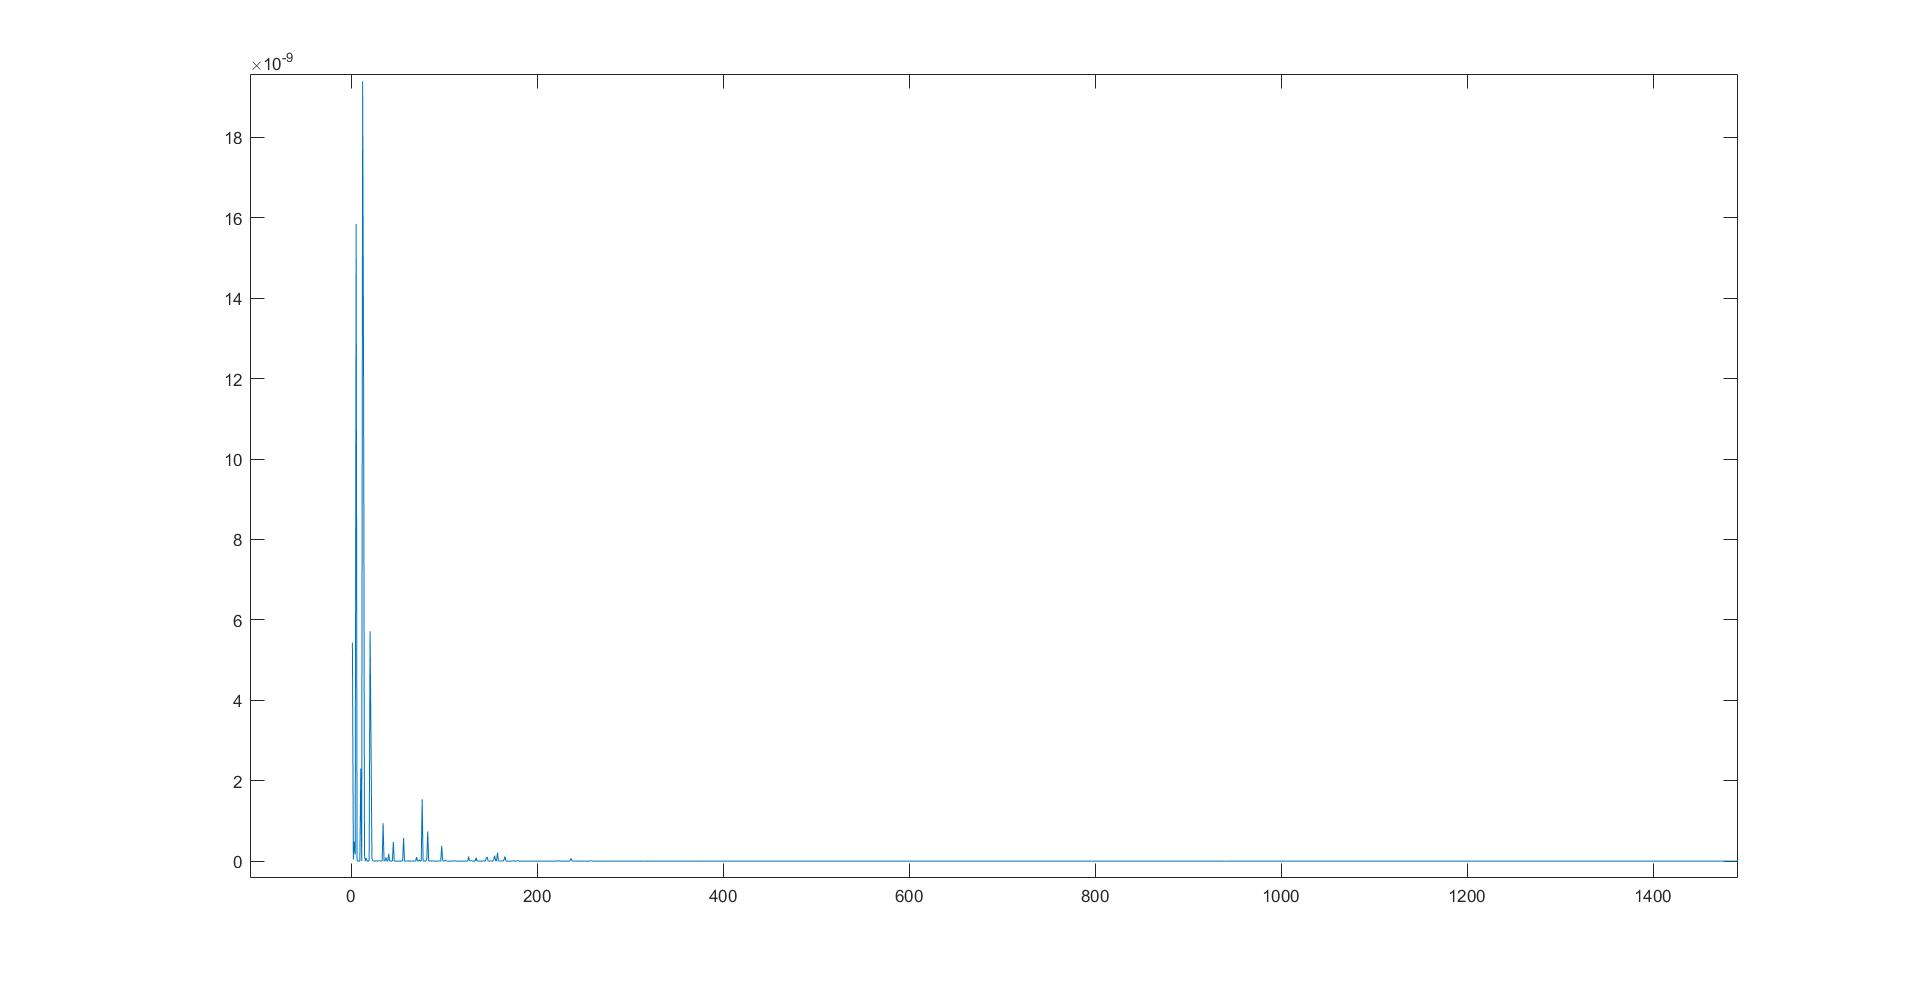
\includegraphics[width=0.8\linewidth]{A3图片/prob.jpg}}
\caption{概率分布图像}
\label{prob}
\end{figure}
最大的概率为1.9397e-08,排列组合为4,9,10,7,8,1,2,6,3,5,这个排列下原本的总用时为197.9792分钟。其他的数值如表\ref{缩短时间}所示
\begin{table}[!ht]
    \centering
    \resizebox{\textwidth}{!}{
    \begin{tabular}{|c|c|c|c|c|c|}
    \hline
        生产的疫苗种类 & 4 & 9 & 10 & 7 & 8 \\ \hline
        需要缩短时间的机器 & 1 & 1 & 1 & 1 & 4 \\ \hline
        每个工位的时间缩短量 & 1.948250626 & 1.882071344 & 0.463695673 & 1.837289751 & 0.522169544 \\ \hline
        每个工位最大的缩短时间量 & 7.988652 & 4.987232 & 0.886396 & 4.149166 & 0.97322 \\ \hline
    \end{tabular}
    }
    ~\\
    ~\\
    \resizebox{\textwidth}{!}{
    \begin{tabular}{|c|c|c|c|c|c|}
    \hline
        生产的疫苗种类 & 1 & 2 & 6 & 3 & 5 \\ \hline
        需要缩短时间的机器 & 1 & 4 & 4 & 2 & 4 \\ \hline
        每个工位的时间缩短量 & 0.767678668 & 1.338403867 & 1.610397238 & 0.017997072 & 1.391130316 \\ \hline
        每个工位最大的缩短时间量 & 1.304306 & 2.023252 & 2.627626 & 0.035944 & 2.11118 \\ \hline
    \end{tabular}
    }
    \caption{缩短所需时间的各个数值}
    \label{缩短时间}
\end{table}\par
后面,我们又带入了缩短比例为1\%到9\%的等间距50个点对所有排列求最大概率,得到如下所示的图像:
\begin{figure}[H]
\centering
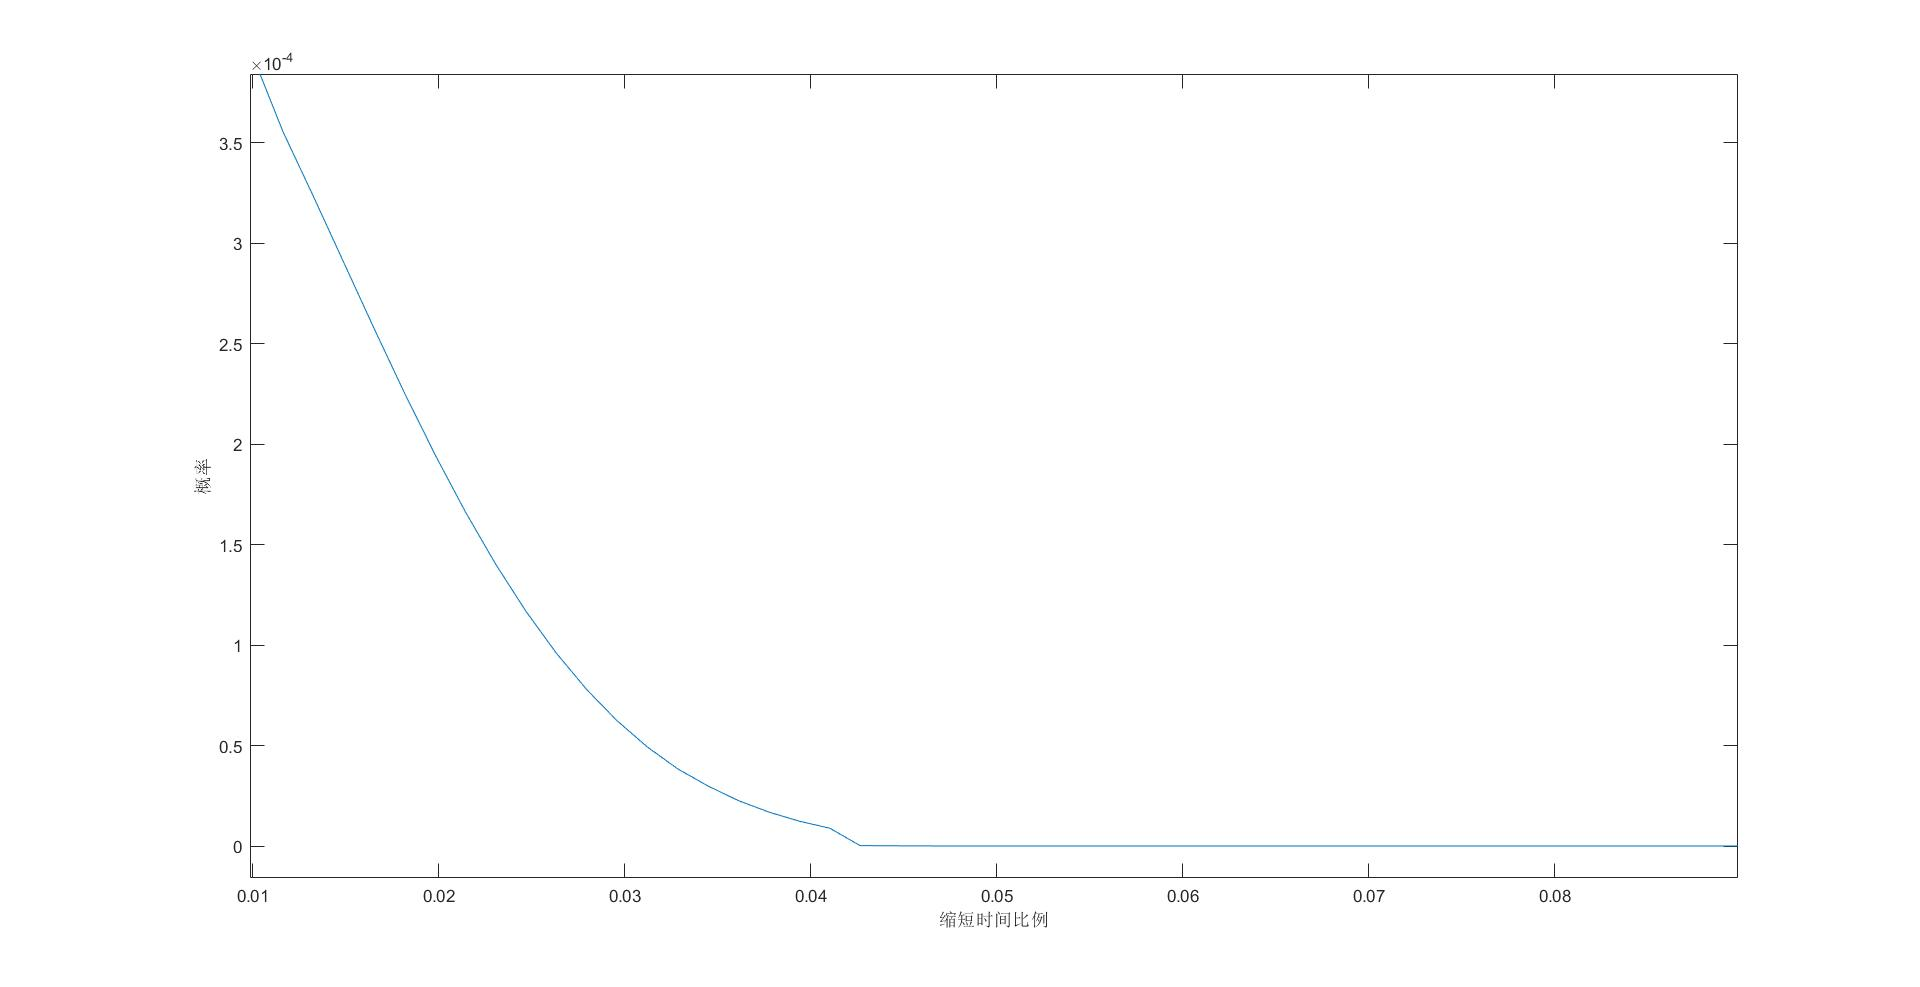
\includegraphics[width=0.8\linewidth]{A3图片/pprob.jpg}
\caption{缩减时间比例与最大概率的关系图}
\label{r-prob-ratio}
\end{figure}

\subsection{问题四模型的建立与求解}
\subsubsection{问题四模型的建立}
对于问题四,该疫苗生产公司接收了10种类型疫苗不同规模的生产任务,且每个工位每天生产的时间不能超过16小时即960分钟。而且同种类型疫苗生产全部完成之后才能生产另外类型的疫苗。对于90\%的可靠性,我们采用正态分布的0.9分位数进行最大值估计。而对于整体规划,由于一次只能先把某种疫苗生产完才可以进行下一个疫苗的生产,且每个疫苗需求量足够大,我们把整个过程分程单独与混合两个阶段进行分析以简化所得的模型。

\begin{wrapfigure}[12]{r}{0.6\textwidth}%数字来规定行数
\vspace{-1em}
  \begin{center}
    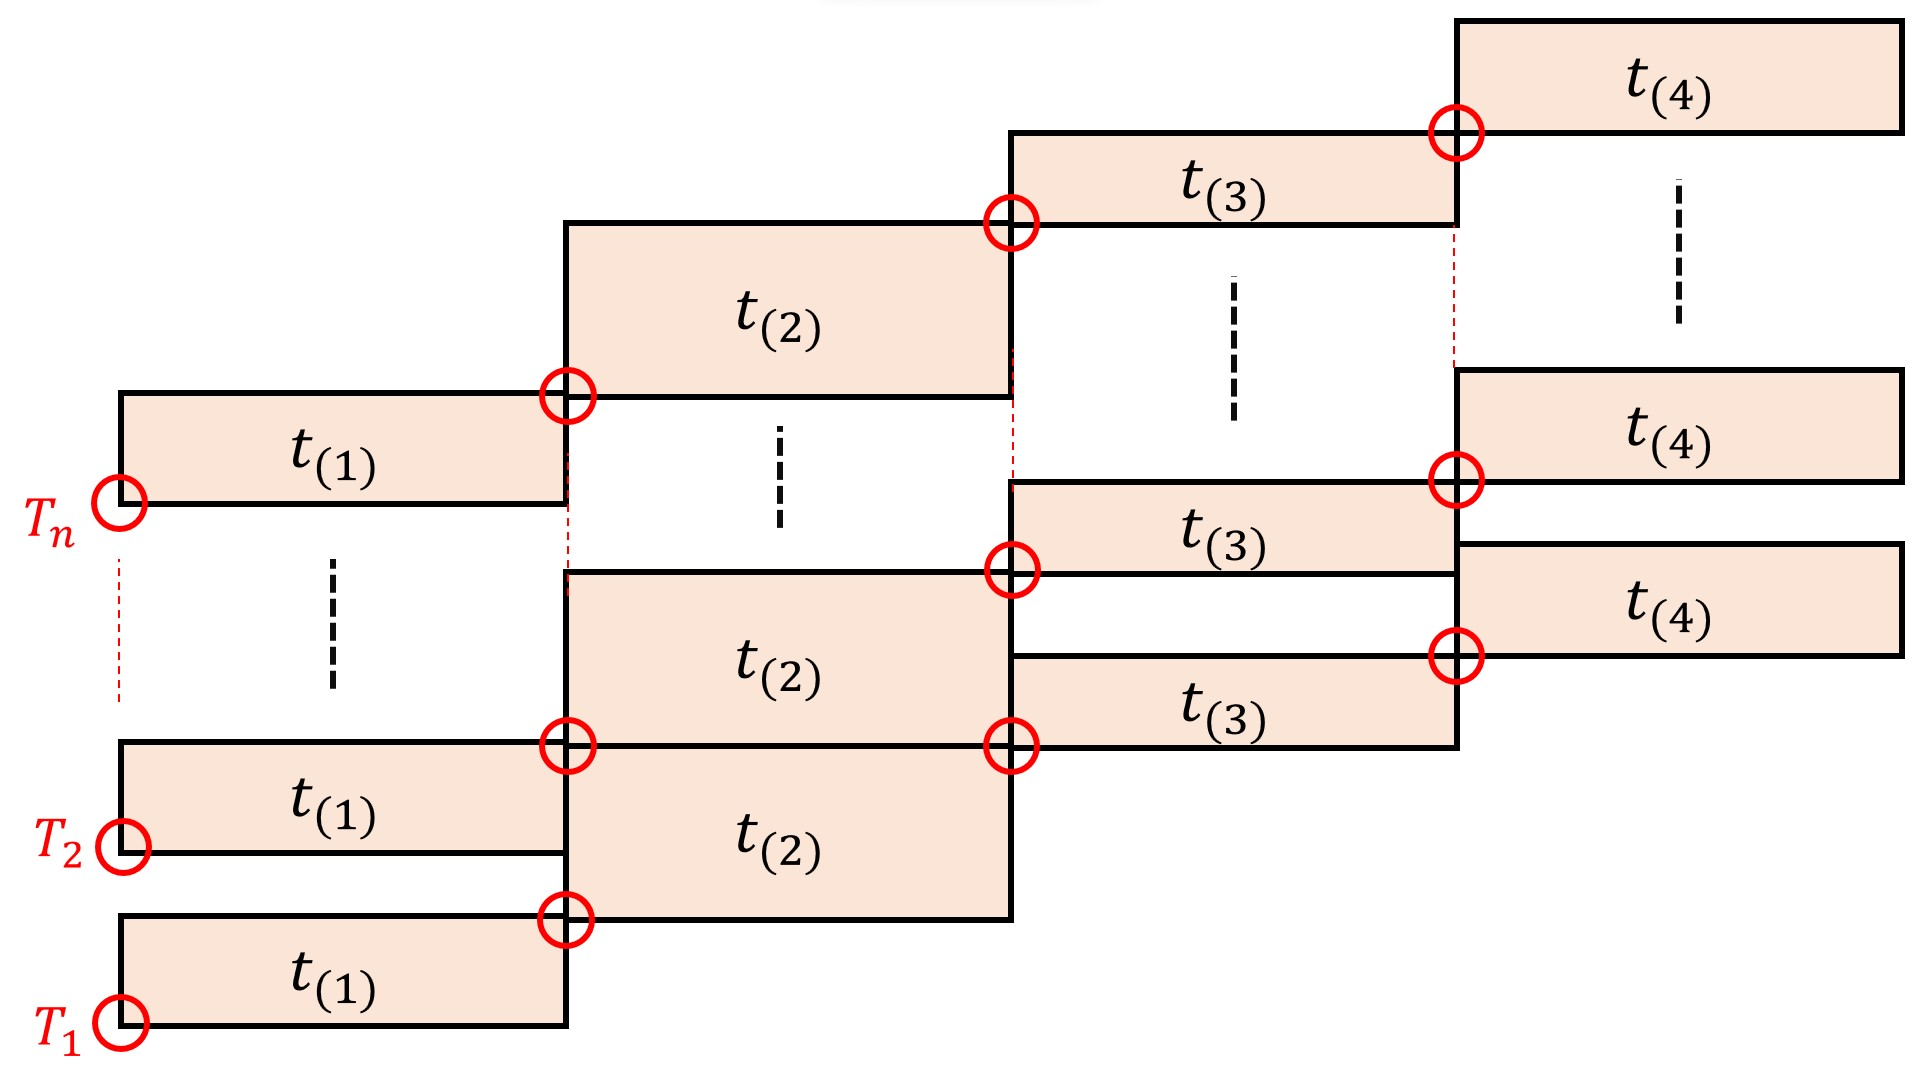
\includegraphics[width=0.6\textwidth]{A4图片/A4pre.JPG}
  \end{center}
  \label{min}
  \caption{最短用时排列模型展示}
\end{wrapfigure}
\textbf{单独过程}:此过程中,一天只生产一个种类的商品,如模型一所示,但所有疫苗种类一致,我们可以看到,如果即如图所示时间点为$T_1$到$T_n$可见,对$1,2,3,4$这四个机器,工作时长都是$T_n - T_1$,且由图可知$T_n - T_1 = (n-1)max(t_i)$.可知每台机器的工作时长为$(n-1)max(t_i)+t_i$且都不超过960分钟,由于前面的为生产完成会导致后面的无法生产,可以知道,只要$n*max(t_i)$不超过960分钟即可。所以每天生产的箱数可以用$[\frac{960}{max \{t_{a(i),j}\} }-0.5]$来表示。\par
\textbf{混合过程}:此过程中由上一种疫苗未完成的部分与下一种疫苗的开始部分组成,此过程中,我们设计了MODEL1函数来进行计算,input上一部分剩余箱数rest,以及上一种与下一种类型的疫苗$a(i),a(i+1)$就可以得到生产的下一种类型疫苗的箱数,算法的思路同问题一,计算出交接处的时间变化再进行计算。\par
将这个问题简化成了两个过程后,大大降低了计算中的复杂度,下面建立动态规划模型

\begin{algorithm}[H]
  \SetAlgoLined
  \KwData{附件1,附件2}
  \KwResult{$min \{D_{total}\}$}
  \While{$max \{Need_{a(i)}\} > 0$}{
    \eIf{$i < 10$}{
      第i类疫苗每天最多生产箱数$P_i = [\frac{960}{max \{t_{a(i),j}\} }-0.5]$\;
      第i类疫苗的生产天数$D_i = [\frac{Need_{a(i)}}{P_i}]+1$\;
      第i类疫苗剩余的箱数$rest_i = Need_{a(i)} \quad mod \quad P_i$\;
      $n = MODEL1(rest,a(i),a(i+1))$\;
      $Need_{a(i+1)} = Need_{a(i+1)} - n$\;
      }{
      $D_i = \frac{Need_{a(i)}}{P_i}$\;
      }
      总天数$D_{total} = \sum_{i=1}^{10}D_i$\;
    }
  \caption{问题四动态规划模型代码}
\end{algorithm}

\subsubsection{问题四模型的求解}
经过Matlab编程之后,我们求解该动态规划模型,得到了用时最短的时间为202天213.12分钟,该用时的总共有两个排列方式
\begin{itemize}
\centering
    \item 7     2     8     4    10     5     1     9     6     3
    \item 2     7     8     4    10     5     1     9     6     3
\end{itemize}
对于该结果的解释:由于中间每个生产有足够的空隙,所以会产生多种情况使得最后的总时间一样。我们绘制出上述二者具体的生产过程,图像如下所示
\begin{figure}[h]
\centering
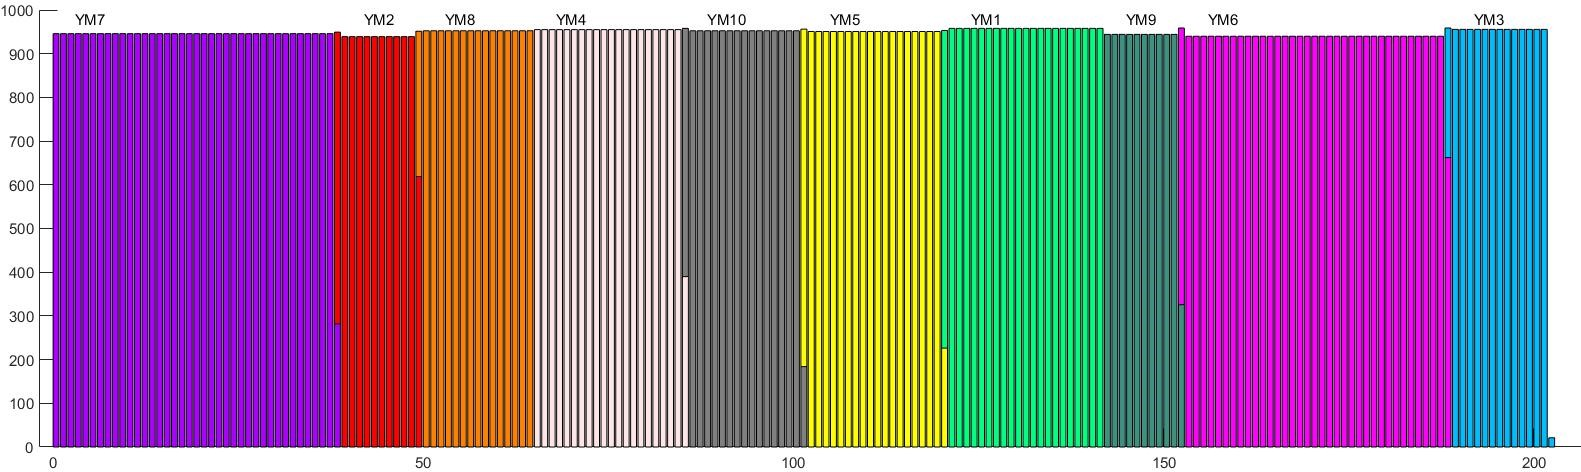
\includegraphics[width=0.8\linewidth]{A4图片/A41.jpg}
\caption{排序为7 2 8 4 10 5 1 9 6 3}
\label{A41}
\end{figure}
\begin{figure}[h]
\centering
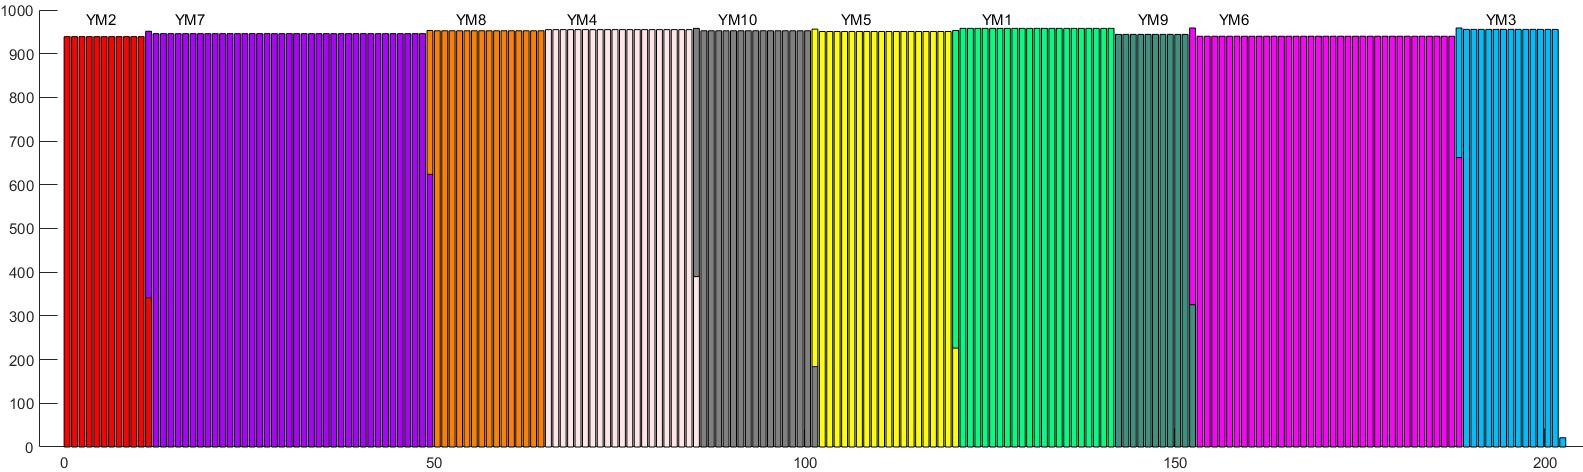
\includegraphics[width=0.8\linewidth]{A4图片/A42.jpg}
\caption{排序为2 7 8 4 10 5 1 9 6 3}
\label{A42}
\end{figure}

\newpage
\subsection{问题五模型的建立与求解}
\subsubsection{问题五模型的建立}
问题五在问题四的基础上增加了可以拆分的条件,即不用把任务全部做完,我们可以计算出每个疫苗的生产性价比$r_{a(i)}$,然后先生产性价比高的,再生产性价比低的,生产到限制的天数100天停止\cite{ref1},记每箱疫苗的售价为$w_{a(i)}$下面我们来分析一下性价比的计算方法:
\begin{align}
    \mbox{每天的生产剂数} =& \frac{960}{max \{t_{a(i),j}\}}\nonumber\\
    \mbox{产生的收益} =& \frac{960}{max \{t_{a(i),j}\}} \times w_{a(i)}\nonumber\\
\end{align}
可见,性价比可以用$\frac{w_{a(i)}}{max \{t_{a(i),j}\}}$来表达,即出售价格除以最长用时,即每单位时间可以带来的的收益。

\subsubsection{问题五模型的求解}
然后,我们用matlab计算出每个疫苗的生产性价比,如下图所示\par
\begin{figure}[h]
\centering
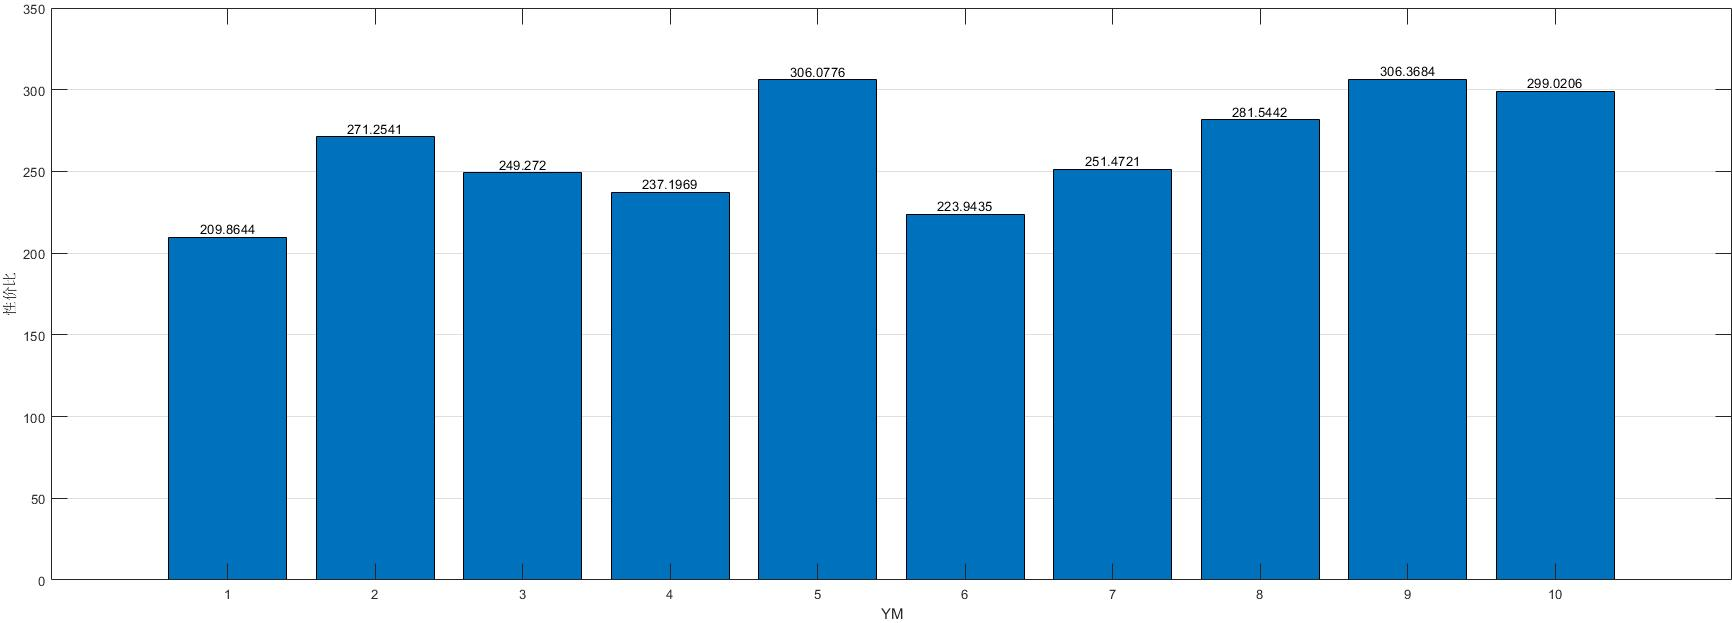
\includegraphics[width=\linewidth]{A4图片/A5pre.jpg}
\caption{性价比排列}
\end{figure}
可见,生产的顺序应该是9 5 10 8 2 7 3 4 6 1,而且前67天可以生产完9到2类型的疫苗,然后再生产33天$YM7$具体的生产利益如下表所示

\begin{table}[!ht]
    \centering
    \begin{tabular}{|c|c|c|c|}
    \hline
        \textbf{生产完天数(天)} & \textbf{疫苗种类} & \textbf{生产该类疫苗用时(天)} & \textbf{生产产生的收入(美元)} \\ \hline
        10 & YM9 & 9+1 & 2760000 \\ \hline
        27 & YM5 & 16+1 & 5040000 \\ \hline
        43 & YM10 & 15+1 & 4320000 \\ \hline
        58 & YM8 & 14+1 & 4080000 \\ \hline
        67 & YM2 & 9 & 2700000 \\ \hline
        100 & YM7 & 33 & 7920000 \\ \hline
        \multicolumn{3}{|c|}{\textbf{总利润}} & 26820000 \\ \hline
    \end{tabular}
    \caption{收入表格}
\end{table}
可见,按照上述表格带来的收益最大,为26820000美元

\newpage
\clearpage
\phantomsection
\addcontentsline{toc}{section}{参考文献}
\tolerance=500
\begin{thebibliography}{99}  
\bibitem{ref1}崔路军.交货期确定条件下的准时制流水车间作业调度问题研究[D].青岛大学,2010.
\bibitem{ref2}王阳.流水车间调度问题的分支定界算法研究[D].辽宁工业大学,2021.DOI:10.27211/d.cnki.glngc.2021.000273.
\end{thebibliography}
\section*{附录}
\addcontentsline{toc}{section}{附录}
\subsection*{A1绘图代码}
\lstinputlisting{code/A1_draw.m}
\subsection*{A2动态规划代码}
\lstinputlisting{code/A2_1_model.m}
\subsection*{A2绘图代码}
\lstinputlisting{code/A2_2_draw.m}
\subsection*{A3数据预处理代码}
\lstinputlisting{code/A3_1_keys.m}
\subsection*{A3记录节点代码}
\lstinputlisting{code/A3_2_record.m}
\subsection*{A3动态规划代码}
\lstinputlisting{code/A3_3_model.m}
\subsection*{A4规划模型代码}
\lstinputlisting{code/A4_1_model.m}
\subsection*{A4绘图代码}
\lstinputlisting{code/A4_2_draw.m}
\subsection*{A5计算代码}
\lstinputlisting{code/A5.m}
\subsection*{cont3函数代码}
\lstinputlisting{code/function_count3.m}
\end{document}



